\documentclass[12pt]{article}
\usepackage{graphicx}     %standard package. Note graphics<graphicx<epsfig
\usepackage{color}     %standard package
\usepackage{hyperref} %standard package written by Sebastian Rahtz
%\usepackage{subeqn}    %allows equations 1a, 1b
%\usepackage{subfig}    %allows figures 1a, 1b
\usepackage{amsmath}
\usepackage{amssymb}
\usepackage{xurl}
\usepackage{bbm}%for indicator function
%\bibliographystyle{alpha}
\usepackage{floatrow}


\usepackage[toc,page]{appendix}
\usepackage[nottoc]{tocbibind}

\usepackage[color,matrix,frame,arrow,curve]{xy}
\usepackage[table,xcdraw]{xcolor}
\usepackage[shortlabels]{enumitem}
\usepackage{array}
\usepackage{pdflscape}
\usepackage{multicol, multirow}
\usepackage{ctable}
\usepackage{dirtree}
\usepackage{subfig}
\usepackage{longtable}

%\usepackage{fdsymbol}
%\usepackage{animate}% play animation

\usepackage[vlined,ruled]{algorithm2e}
\newcommand{\mycommfont}[1]{\small\ttfamily\textcolor{blue}{#1}}
\SetCommentSty{mycommfont}

%highlighting
\usepackage{mdframed}

\usepackage[makeroom]{cancel}

\usepackage{pdfpages}
\usepackage{hyperxmp}

\paperheight=11in
\topmargin=0in
\headheight=0in
\headsep=0in
\topskip=0in
\textheight=8.5in
\footskip=.5in


\paperwidth=8.5in
\oddsidemargin=.25in
\evensidemargin=.25in
\textwidth=6.0in
\parindent=.5in

\newcommand{\chapquote}[3]{\begin{quotation} \textit{#1} \end{quotation} \begin{flushright} - #2, \textit{#3}\end{flushright} }

\newtheorem{claim}{Claim}
\newcommand{\proof}[0]{{\bf proof:} }
\newcommand{\qed}[0]{\quad\newline \noindent{\bf QED }}


\newcommand{\bra}[1]{\langle#1|}
\newcommand{\ket}[1]{|#1\rangle}
\newcommand{\av}[1]{\left\langle#1\right\rangle}
\newcommand{\pder}[2]{\frac{\partial#1}{\partial#2}}
\newcommand{\der}[2]{\frac{d#1}{d#2}}
\newcommand{\tr}[0]{{\rm tr }}
\newcommand{\beq}{\begin{equation}}
\newcommand{\eeq}{\end{equation}}
\newcommand{\bsub}{\begin{subequations}}
	\newcommand{\esub}{\end{subequations}}
\newcommand{\beqa}{\begin{eqnarray}}
\newcommand{\eeqa}{\end{eqnarray}}
\newcommand{\rarrow}[0]{\rightarrow}
\newcommand{\larrow}[0]{\leftarrow}
\newcommand{\uarrow}[0]{\uparrow}
\newcommand{\darrow}[0]{\downarrow}
\newcommand{\Rarrow}[0]{\Rightarrow}
\newcommand{\nRarrow}[0]{\nRightarrow}
\newcommand{\Larrow}[0]{\Leftarrow}
\newcommand{\nLarrow}[0]{\nLeftarrow}
\newcommand{\ul}[1]{\underline{#1}}
\newcommand{\ol}[1]{\overline{#1}}
\newcommand{\ZZ}[0]{ {\mathbb{Z}}}
\newcommand{\RR}[0]{{ \mathbb{R}} }
\newcommand{\CC}[0]{{ \mathbb{C}} }
\newcommand{\XX}[0]{{ \mathbb{X}} }
\newcommand{\ground}{{}_{\stackrel{\stackrel{\displaystyle{\bot}}{-}}{.}}}
\newcommand{\norm}[1]{\parallel#1\parallel}
\newcommand{\eqdef}[0]{\;\;\stackrel{\text{def}}{=}\;\;}

\newcommand{\heavy}[0]{\mathbf{H}}

\newcommand{\rva}[0]{{\ul{a}}}
\newcommand{\rvb}[0]{{\ul{b}}}
\newcommand{\rvc}[0]{{\ul{c}}}
\newcommand{\rvd}[0]{{\ul{d}}}
\newcommand{\rve}[0]{{\ul{e}}}
\newcommand{\rvf}[0]{{\ul{f}}}
\newcommand{\rvg}[0]{{\ul{g}}}
\newcommand{\rvh}[0]{{\ul{h}}}
\newcommand{\rvi}[0]{{\ul{i}}}
\newcommand{\rvj}[0]{{\ul{j}}}
\newcommand{\rvk}[0]{{\ul{k}}}
\newcommand{\rvl}[0]{{\ul{l}}}
\newcommand{\rvll}[0]{{\ul{\ell}}}
\newcommand{\rvm}[0]{{\ul{m}}}
\newcommand{\rvn}[0]{{\ul{n}}}
\newcommand{\rvo}[0]{{\ul{o}}}
\newcommand{\rvp}[0]{{\ul{p}}}
\newcommand{\rvq}[0]{{\ul{q}}}
\newcommand{\rvr}[0]{{\ul{r}}}
\newcommand{\rvs}[0]{{\ul{s}}}
\newcommand{\rvt}[0]{{\ul{t}}}
\newcommand{\rvu}[0]{{\ul{u}}}
\newcommand{\rvv}[0]{{\ul{v}}}
\newcommand{\rvw}[0]{{\ul{w}}}
\newcommand{\rvx}[0]{{\ul{x}}}
\newcommand{\rvy}[0]{{\ul{y}}}
\newcommand{\rvz}[0]{{\ul{z}}}


\newcommand{\rvA}[0]{{\ul{A}}}
\newcommand{\rvB}[0]{{\ul{B}}}
\newcommand{\rvC}[0]{{\ul{C}}}
\newcommand{\rvD}[0]{{\ul{D}}}
\newcommand{\rvE}[0]{{\ul{E}}}
\newcommand{\rvF}[0]{{\ul{F}}}
\newcommand{\rvH}[0]{{\ul{H}}}
\newcommand{\rvK}[0]{{\ul{K}}}
\newcommand{\rvL}[0]{{\ul{L}}}
\newcommand{\rvN}[0]{{\ul{N}}}
\newcommand{\rvQ}[0]{{\ul{Q}}}
\newcommand{\rvR}[0]{{\ul{R}}}
\newcommand{\rvT}[0]{{\ul{T}}}
\newcommand{\rvU}[0]{{\ul{U}}}
\newcommand{\rvV}[0]{{\ul{V}}}
\newcommand{\rvW}[0]{{\ul{W}}}
\newcommand{\rvX}[0]{{\ul{X}}}
\newcommand{\rvY}[0]{{\ul{Y}}}
\newcommand{\rvZ}[0]{{\ul{Z}}}

\newcommand{\rvxi}[0]{{\ul{\xi}}}
\newcommand{\rvzeta}[0]{{\ul{\zeta}}}
\newcommand{\rvtheta}[0]{{\ul{\theta}}}
\newcommand{\rvmu}[0]{{\ul{\mu}}}
\newcommand{\rvsig}[0]{{\ul{\sigma}}}
\newcommand{\rvDel}[0]{{\ul{\Delta}}}
\newcommand{\rvtau}[0]{{\ul{\tau}}}

\newcommand{\cala}[0]{{\cal A}}
\newcommand{\calb}[0]{{\cal B}}
\newcommand{\calc}[0]{{\cal C}}
\newcommand{\cald}[0]{{\cal D}}
\newcommand{\cale}[0]{{\cal E}}
\newcommand{\calf}[0]{{\cal F}}
\newcommand{\calg}[0]{{\cal G}}
\newcommand{\calh}[0]{{\cal H}}
\newcommand{\cali}[0]{{\cal I}}
\newcommand{\calk}[0]{{\cal K}}
\newcommand{\call}[0]{{\cal L}}
\newcommand{\calm}[0]{{\cal M}}
\newcommand{\caln}[0]{{\cal N}}
\newcommand{\calo}[0]{{\cal O}}
\newcommand{\calp}[0]{{\cal P}}
\newcommand{\calq}[0]{{\cal Q}}
\newcommand{\calr}[0]{{\cal R}}
\newcommand{\cals}[0]{{\cal S}}
\newcommand{\calt}[0]{{\cal T}}
\newcommand{\calu}[0]{{\cal U}}
\newcommand{\calv}[0]{{\cal V}}
\newcommand{\calw}[0]{{\cal W}}
\newcommand{\calx}[0]{{\cal X}}
\newcommand{\caly}[0]{{\cal Y}}
\newcommand{\calz}[0]{{\cal Z}}

\newcommand{\Pmat}[4]{\calp\left[
\begin{array}{cc}#1&#2\\#3&#4
\end{array}\right]}

%\newcommand{\PN}[0]{PN^{0,0}_{1,1}}
%\newcommand{\PS}[0]{PS^{1,1}_{0,0}}
\newcommand{\PN}[0]{PN}
\newcommand{\PS}[0]{PS}

\newcommand{\lam}[0]{\lambda}
\newcommand{\Lam}[0]{\Lambda}
\newcommand{\alp}[0]{\alpha}
\newcommand{\eps}[0]{\epsilon}
\newcommand{\s}[0]{\sigma}
\newcommand{\su}[0]{{\Sigma}}

\newcommand{\pp}[0]{\mathbb{P}}
\newcommand{\dbm}[0]{{
		[1,\partial_{b},\partial_{m}]
}}

\newcommand{\dg}[0]{{[1, \partial_{\theta_G}]}}
\newcommand{\dd}[0]{{[1, \partial_{\theta_D}]}}
\newcommand{\dgd}[0]{{[1, \partial_{\theta_G}, \partial_{\theta_D}]}}

\newcommand{\veca}[0]{{\vec{a}}}
\newcommand{\vecb}[0]{{\vec{b}}}
\newcommand{\vecc}[0]{{\vec{c}}}
\newcommand{\vecd}[0]{{\vec{d}}}
\newcommand{\vecf}[0]{{\vec{f}}}
\newcommand{\vech}[0]{{\vec{h}}}
\newcommand{\vecr}[0]{{\vec{r}}}
\newcommand{\vecs}[0]{{\vec{s}}}
\newcommand{\vecu}[0]{{\vec{u}}}
\newcommand{\vecx}[0]{{\vec{x}}}
\newcommand{\vecy}[0]{{\vec{y}}}
\newcommand{\vechy}[0]{{\vec{\haty}}}
\newcommand{\vtheta}[0]{{\vec{\theta}}}

\newcommand{\haty}[0]{{\widehat{y}}}
\newcommand{\hatx}[0]{{\widehat{x}}}
\newcommand{\hata}[0]{{\widehat{a}}}
\newcommand{\hatr}[0]{{\widehat{r}}}


\newcommand{\cond}[0]{{\:\mathbf{|}\:}}
\newcommand{\mymathbf}[1]{#1}

\newcommand{\ranvec}[1]{\ul{\vec{#1}}}
\newcommand{\indi}[0]{\mathbbm{1}}
\newcommand{\smoid}[0]{{\rm smoid}}
\newcommand{\lodds}[0]{{\rm lodds}}
\newcommand{\expit}[0]{{\rm expit}}
\newcommand{\logit}[0]{{\rm logit}}
\newcommand{\sign}[0]{{\rm sign}}

\renewcommand{\labelitemii}{$\bullet$}

\newcommand{\HAT}[1]{{\widehat{#1}}}
\newcommand{\TIL}[1]{{\widetilde{#1}}}
\newcommand{\tild}[0]{{\TIL{d}}}
\newcommand{\tile}[0]{{\TIL{e}}}
\newcommand{\tilg}[0]{{\TIL{g}}}
\newcommand{\tilu}[0]{{\TIL{u}}}
\newcommand{\tilx}[0]{{\TIL{x}}}
\newcommand{\tilP}[0]{{\TIL{P}}}
\newcommand{\tilPT}[0]{{\TIL{P}_\theta}}

\newcommand{\maparrow}[1]
{\xymatrix{\ar[r]_{#1}&}}


\newcommand{\ucalm}[0]{\ul{\calm}}

\newcommand{\bool}[0]{\{0,1\}}

\newcommand{\argmin}{\mathop{\mathrm{argmin}}\limits}
\newcommand{\argmax}{\mathop{\mathrm{argmax}}\limits}

\newcommand{\softmax}[0]{{\rm softmax}}

\newcommand{\A}[0]{\wedge}
\newcommand{\V}[0]{\vee}
\newcommand{\xor}{\oplus}
\newcommand{\bigA}[0]{\bigwedge}
\newcommand{\bigV}[0]{\bigvee}
\newcommand{\bigxor}{\bigoplus}


\newcommand{\rdart}[0]{\Rightarrow}
\newcommand{\ldart}[0]{\Leftarrow}
\newcommand{\rveps}[0]{\ul{\eps}}

\newcommand{\hatvar}[0]{\widehat{\sigma^2}}
\newcommand{\ptp}[0]{{(t)}}

\newcommand{\tseries}[1]{{\{#1\}_{\forall t}}}

\newcommand{\xbeta}[0]{X_\s^T\beta}
\newcommand{\xtau}[0]{X_\s^T\tau}

%arguments phi1, phi2, phi3, e
\newcommand{\rbd}[4]{
\xymatrix@-1.3pc{
&#1\ar[d]&&#2\ar[d]
\\
&\rvx_1\ar[rr]
&&
\rvx_2
\ar `r[rd][rd]
\\
0\ar`u[u][ru]
\ar`d[dr][rrd]
&&&&\rvA\ar[r]&#4
\\
&&
\rvx_3
\ar `r[rru][rru]
\\
&&#3\ar[u]
}
}

\newcommand{\rulezeroif}[0]{
If $(\rvb. \perp \rva.
|\rvr., \rvs.)$
in $G$, then}

\newcommand{\rulezerothen}[0]{
$\rva.=a. \leftrightarrow 1$}

\newcommand{\rulezeroP}[0]{
P(b.|a.,r.,s.)=P(b.|r., s.)}

\newcommand{\rulezeroH}[0]{
H(\rvb.:\rva.|\rvr.,\rvs.)=0}

\newcommand{\rulezeropic}[0]{
\xymatrix@C=1pc@R=1pc{
&r.\ar[dr]
&s.\ar[d]
\\
a.\ar[rr]
&&b.
&=
}
\xymatrix@C=1pc@R=1pc{
&r.\ar[dr]&s.\ar[d]
\\
a.\ar[rr]|0
&&b.
}}

\newcommand{\ruleoneif}[0]{
If $(\rvb. \perp \rva.
|\rvr., \rvs.)$
in $\cald_{\rvr.} G$, then}

\newcommand{\ruleonethen}[0]{
$\rva.=a. \leftrightarrow 1$}

\newcommand{\ruleoneP}[0]{
P(b.|a., \cald\rvr.=r.,s.)=
P(b.|\cald\rvr.=r., s.)}

\newcommand{\ruleoneH}[0]{
H(\rvb.:\rva.|\cald\rvr.,\rvs.)=0}

\newcommand{\ruleonepic}[0]{
\xymatrix@C=1pc@R=1pc{
&\cald\rvr.=r.\ar[dr]
&s.\ar[d]
\\
a.\ar[rr]
&&b.
&=
}
\xymatrix@C=1pc@R=1pc{
&\cald\rvr.=r.\ar[dr]
&s.\ar[d]
\\
a.\ar[rr]|0
&&b.
}}

\newcommand{\ruletwoif}[0]{
If $(\rvb.\perp \rva. |
 \rvr., \rvs.)$
in $\call_{\rva.}\cald_{\rvr.} G$,
 then}

\newcommand{\ruletwothen}[0]{
$\cald \rva.=a. \leftrightarrow \rva.=a.$}

\newcommand{\ruletwoP}[0]{
P(b.|\cald\rva.=a., \cald\rvr.=r., s.)=
P(b.|a., \cald\rvr.=r.,  s.)}

\newcommand{\ruletwoH}[0]{
H(\rvb.:\cald\rva.|\cald\rvr.,  \rvs.)
=
H(\rvb.:\rva.|\cald\rvr.,  \rvs.)}

\newcommand{\ruletwopicA}[0]{
\xymatrix@C=1pc@R=1pc{
\;\ar[d]_0
&\cald\rvr.=r.\ar[dr]
&s.\ar[d]
\\
\cald\rva.=a.\ar[rr]\ar[d]
&&b.
&=\quad\quad
\\
&
}
\xymatrix@C=1pc@R=1pc{
\;\ar[d]_0
&&\cald\rvr.=r.\ar[dr]
&s.\ar[d]
\\
\cald\rva.=a.\ar[d]
&a.\ar[rr]
&&b.
\\
&
}}
\newcommand{\ruletwopicB}[0]{
\xymatrix@C=1pc@R=1pc{
\;\ar[d]
&\cald\rvr.=r.\ar[dr]
&s.\ar[d]
\\
a.\ar[rr]\ar[d]
&&b.
&=\quad\quad
\\
&
}
\xymatrix@C=1pc@R=1pc{
\;\ar[d]
&&\cald\rvr.=r.\ar[dr]
&s.\ar[d]
\\
a.\ar[d]
&\cald\rva.=a.\ar[rr]
&&b.
\\
&
}}

\newcommand{\rulethreeif}[0]{
If $
(\rvb. \perp \rva.
| \rvr., \rvs.)$
in $\cald_{\rva.-an(\rvs.)}
\cald_{\rvr.}G$,
 then}

\newcommand{\rulethreethen}[0]{
$\cald \rva.=a. \leftrightarrow 1$}

\newcommand{\rulethreeP}[0]{
P(b.|\cald\rva.=a.,\cald\rvr.=r.,  s.)=
P(b.|\cald\rvr.=r., s.)}

\newcommand{\rulethreeH}[0]{
H(\rvb.:\cald\rva.|\cald\rvr., \rvs.)=0}

\newcommand{\rulethreepic}[0]{
\xymatrix@C=1pc@R=1pc{
&
&\cald\rvr.=r.\ar[dr]
&s.\ar[d]
\\
&\cald\rva.=a.\ar[rr]
&&b.
&=
}
\xymatrix@C=1pc@R=1pc{
&
&\cald\rvr.=r.\ar[dr]
&s.\ar[d]
\\
&\cald\rva.=a.\ar[rr]|0
&&b.
}}

\newcommand{\bdoordef}[0]{
Suppose that we have access to data
that allows us to
estimate a probability
distribution
 $P(x., y., z.)$.
Hence, the variables
$\rvx., \rvy., \rvz.$ are
ALL observed (i.e, not hidden).
Then we say that the
backdoor $\rvz.$
satisfies the
{\bf backdoor adjustment criterion}
relative to $(\rvx., \rvy.)$
if
\begin{enumerate}
\item
All backdoor paths from $\rvx.$
to $\rvy.$
 are blocked by  conditioning on
 $\rvz.$.
\item
$\rvz. \cap de(\rvx.)=\emptyset$.
\end{enumerate}
}

\newcommand{\bdoorclaim}[0]{
If $\rvz.$ satisfies the
backdoor criterion relative to
 $(\rvx., \rvy.)$, then

\beqa
P(y. | \cald \rvx.=x.)&=&
\sum_{z.} P(y.|x., z.)P(z.)
\\
&=&
\begin{array}{l}
\\
\\
\end{array}
\xymatrix{
\sum z.\ar[dr]
\\
x.\ar[r]
&y.
}
\eeqa
where $\sum z.$ means node
$\rvz.$ is summed over.
}

\newcommand{\fdoordef}[0]{
Suppose that we have access to data
that allows us to
estimate a probability
distribution
 $P(x., m., y.)$.
Hence, the variables
$\rvx., \rvm., \rvy.$ are
ALL observed (i.e, not hidden).
Then we say that
the frontdoor $\rvm.$
satisfies the
{\bf frontdoor adjustment criterion}
relative to $(\rvx., \rvy.)$
if
\begin{enumerate}
\item
All directed paths from
$\rvx.$ to $\rvy.$ are intercepted by
(i.e., have a node in) $\rvm.$.
\item
All backdoor paths from $\rvx.$ to
$\rvm.$ are blocked.
\item
All backdoor paths from
on $\rvm.$ to $\rvy.$
are blocked by conditioning
on  $\rvx.$.
\end{enumerate}
}

\newcommand{\fdoorclaim}[0]{
If $\rvm.$ satisfies the
frontdoor criterion
relative to $(\rvx., \rvy.)$,
and $P(x.,m.)>0$, then

\beqa
P(y. | \cald \rvx.=x.)&=&\sum_{m.}
\underbrace{\left[\sum_{x'.}
P(y.|x'., m.)P(x'.)\right]}_
{P(y.|\cald \rvm.=m.)}
\underbrace{P(m.|x.)}_
{P(m.|\cald \rvx.=x.)}
\\
&=&
\xymatrix{
&\sum x'.\ar[dr]
\\
x.´\ar[r]
&\sum m.\ar[r]&y.
}
\eeqa
where $\sum x'.$ and
$\sum m.$
means nodes
$\rvx'.$ and $\rvm.$
are summed over.
}


%Symmetry
\newcommand{\symrule}[0]{
$\rva\perp_P\rvb\implies \rvb\perp_P\rva$}

\newcommand{\symruleH}[0]{
$H(\rva:\rvb)=0\implies H(\rvb:\rva)=0$}

%Decomposition
\newcommand{\decrule}[0]{
$\rva\perp_P\rvb, \rvc\implies
\rva\perp_P\rvb \text{ and } \rva\perp_P\rvc$}

\newcommand{\decruleH}[0]{
$H(\rva:\rvb, \rvc)=0\implies
H(\rva:\rvb)=0 \text{ and } H(\rva:\rvc)=0$}

%Weak Union
\newcommand{\wearule}[0]{
$\rva\perp_P \rvb, \rvc \implies
\rva\perp_P\rvb|\rvc\text{ and }\rva\perp_P\rvc|\rvb$}

\newcommand{\wearuleH}[0]{
$H(\rva:\rvb, \rvc)=0 \implies
H(\rva:\rvb|\rvc)=0\text{ and }H(\rva:\rvc|\rvb)=0$}

%Contraction
\newcommand{\conrule}[0]{
$\rva\perp_P\rvb|\rvc\text{ and }\rva\perp_P \rvc
\implies \rva\perp_P \rvb, \rvc$}

\newcommand{\conruleH}[0]{
$H(\rva:\rvb|\rvc)=0\text{ and }H(\rva:\rvc)=0
\implies H(\rva:\rvb, \rvc)=0$}

%Intersection
\newcommand{\intrule}[0]{
$\rva\perp_P\rvb|\rvc, \rvd\text{ and }
\rva\perp_P \rvd|\rvc, \rvb\implies
\rva\perp_P \rvb,\rvd|\rvc$}

\newcommand{\intruleH}[0]{
$H(\rva:\rvb|\rvc, \rvd)=0\text{ and }
H(\rva:\rvd|\rvc, \rvb)=0\implies
H(\rva:\rvb,\rvd|\rvc)=0$}

\newcommand{\dotbarmu}[0]{{\cdot|\mu}}
\newcommand{\dotmu}[0]{{\cdot, \mu}}
\newcommand{\kbarmu}[0]{{k|\mu}}
\newcommand{\kmu}[0]{{k,\mu}}
\newcommand{\plusbarmu}[0]{{+|\mu}}
\newcommand{\plusmu}[0]{{+,\mu}}

\newcommand{\bnlearn}[0]{{\tt bnlearn\;}}

\newcommand{\sqsig}[0]{{[\sigma]}}

\newcommand{\misscellone}[0]{
\begin{array}{c}
\frac{1}{nsam}
P(x_0=0, x_2=0\cond x_1=1, \theta)
\\
\frac{1}{nsam}
P(x_0=0, x_2=1\cond x_1=1, \theta)
\\
\frac{1}{nsam}
P(x_0=1, x_2=0\cond x_1=1, \theta)
\\
\frac{1}{nsam}
P(x_0=1, x_2=1\cond x_1=1, \theta)
\end{array}
}

\newcommand{\misscelltwo}[0]{
\begin{array}{c}
\frac{1}{nsam}
P(x_1=0\cond x_0=0,x_2=1, \theta)
\\
\frac{1}{nsam}
P(x_1=1\cond x_0=0,x_2=1,  \theta)
\end{array}
}


\newcommand{\td}[0]{{\TIL{d}}}
\newcommand{\rvtd}[0]{{\ul{\TIL{d}}}}
\newcommand{\tx}[0]{{\TIL{x}}}
\newcommand{\tmu}[0]{{\TIL{\mu}}}
\newcommand{\rvtx}[0]{{\ul{\TIL{x}}}}

\newcommand{\mlarr}[0]{\xrightarrow{\rm ML-fit}}
\newcommand{\lrarr}[0]{\xrightarrow{\rm LR-fit}}

\newcommand{\setprob}[3]
{{\begin{array}{c}S=\{#1\}
\\P(S)=#2\\ \haty(x^\s_S)=\$#3 K
\end{array}}}

\newcommand{\Gno}[0]{\xymatrix{\;\ar[r]|\parallel_G&}}
\newcommand{\Gyes}[0]{\xymatrix{\;\ar[r]_G&}}

\newcommand{\calypso}[0]{\ol{\caly}}

\newcommand{\SeqBdoorDef}[0]{
Suppose that we have access to data
that allows us to
estimate a probability
distribution
 $P(x^n, y, z^n)$.
Hence, the variables
$\rvx^n, \rvy, \rvz^n$ are
ALL observed (i.e, not hidden).
Then we say that the
the multinode
of ``covariates" $\rvz^n$
satisfies the
{\bf sequential backdoor (SBD) adjustment criterion}
relative to $(\rvx^n, \rvy)$
if for all $t\in\{0,1, \ldots, n-1\}$,

\begin{enumerate}
\item
$\rvy\perp\rvx_t|
\underbrace{(\rvx_0, \rvx_1, \ldots,\rvx_{t-1},
\rvz_0, \rvz_1, \ldots, \rvz_t)}
_{\text{Past of $\rvx_t$}}$
in $\call_{\rvx_{t}}
\cald_{\rvx_{t+1},\rvx_{t+2}
,\ldots, \rvx_{n-1}}G$.
\item
$\rvz_t \cap de(\rvx_t)=\emptyset$.
\end{enumerate}
}

\newcommand{\SeqBdoorClaim}[0]{
If $\rvz^n$ satisfies the
sequential backdoor criterion relative to
 $(\rvx^n, \rvy)$, then

\beq
P(y | \cald \rvx^n=x^n)=
\calq(y|x^n)
\;,
\eeq
where $\calq(y|x^n)$
is defined by
Eq.(\ref{def-q-y-xn-seqbdoor}).
}



\begin{document}
\title{Causal DAG Extraction from 3 Short Stories  \\
and 3 Movie Scripts (V2)}
\date{ \today}
\author{Robert R. Tucci\\
        tucci@ar-tiste.com}
\maketitle
\vskip2cm
\section*{Abstract}
I improve an algorithm previously
proposed by me 
for doing causal DEFT (DAG Extraction from Text), and then I apply the new algorithm to 2 usecases:
3 short stories by P.G. Wodehouse and 3 movie scripts by Pixar/Disney. The software  used to accomplish this 
endeavor is called ``Mappa Mundi" (MM) and is available as open source at
GitHub.
I discuss possible ways of improving the MM algorithm
using LLMs (Large
Language Models such as ChatGPT).
I also travel this road in the opposite direction---I discuss possible ways of improving
LLMs using the Mappa Mundi algorithm.
\newpage

\chapquote{``If humans were so good at causal inference, religion would not exist."}
{Yann LeCun}{Ref.\cite{yann-religion}}

\chapquote{``How much of human knowledge is captured in all the text ever written? To which my answer is: not much.
"}{Yann LeCun}{Ref.\cite{yann-text}}
\section{Introduction}


In this paper, I improve an algorithm
for doing causal DEFT (DAG Extraction from Text)
that was
first proposed by me in Ref.\cite{deft1}
I then apply the new algorithm to 2 usecases:
\begin{enumerate}

\item 3 short stories by P.G. Wodehouse
(the text for these was obtained from the
Project Gutenberg website Ref.\cite{project-gutenberg}) 

\begin{itemize}
\item  Bill the Bloodhound
\item  Extricating Young Gussie
\item Wilton's Holiday
\end{itemize}

\item 3 movie scripts by Pixar/Disney.
(the text for these was obtained from the IMSDb website
Ref.\cite{imsdb})\footnote{The Mappa Mundi repo at GitHub
contains a Python script called {\tt downloading.py}
that uses the BeautifulSoup Python
package to scrape all the $1100+$ movie
scripts available (about 230 MB) at the IMSDb website.
My original intention
was to apply my algorithm to 
all of those movie scripts.
However, due to lack of
hardware resources, I had to 
settle for just 3 movie scripts.}

\begin{itemize}
\item Toy Story 
\item Up
\item WALL-E
\end{itemize}
\end{enumerate}

The Python 
software that was used to 
accomplish this endeavor is 
called Mappa Mundi (MM). It is open source and available
at GitHub (Ref.\cite{github-mappa-mundi}).



So what is MM good for? The goal of DEFT in general and MM in particular, is to create a directory 
of DAGs (``DAG atlas").
Conjecturing
a DAG is always the first step
in doing Judea Pearl's causal inference (CI).\footnote{Judea Pearl's CI is described
in detail in Pearl's {\it The Book of Why}
(Ref.\cite{book-of-why})
and in my free, open source book {\it Bayesuvius} (Ref. \cite{bayesuvius}).}
Once a DAG is available,
one can use it to 
do Pearl's 3 rungs of CI,
using tools such as SCuMpy.\footnote{DAG = Directed Acyclic Graph, SCM = Structural Causal Model, a type of DAG}\footnote{Shameless plug: my free, open source software
SCuMpy (Ref.\cite{scumpy})
can be used to do all 3 rungs
of CI. 
It can handle all types of linear SCM, including
SCM with feedback loops and hidden variables.} 

As I explained in my previous paper Ref.\cite{deft1}, the scientific method (SM) looks for causation, not correlation. Pearl CI is the gold standard theory for distinguishing
between correlation and causation.
Hence, the SM and Pearl CI are closely related.
Pearl CI can be viewed as an application of the SM, wherein the DAG is the hypothesis part of the SM---what we want to  
prove or disprove.
DEFT provides DAG hypotheses.
For example,
DEFT could be used to discover causal DAGs that indicate pathways to diseases.

At the end of this paper, I discuss possible ways of improving the MM algorithm 
using LLMs (Large
Language Models such as ChatGPT).
I also travel this road in the opposite direction---
I discuss
possible ways of improving
LLMs using the MM algorithm.


\section{MM Algorithm Overview}
\label{sec-algo-overview}
The MM algorithm proposed in this
paper can be applied to a broad range of texts. The only constraint is that those texts 
do ``story-telling" in a chronological order.
That is why I decided to use movie scripts,
because movie-scripts usually do story-telling in a chronological order (except when they do 
flashbacks or time travel, but that isn't very
common in movies.)

The MM algorithm would not work well
if applied to the corpus of science papers at arXiv,
because scientific papers normally don't do chronological story-telling. 
On the other hand,
it might work well if applied to a corpus of (time stamped) lab notebooks maintained by one or more experimental scientists.
It might also work well on a corpus of time-stamped logs maintained by one or more person
trying to figure out the cause of a disease.

The MM algorithm would also
work well on a corpus of videos or movies that
do chronological story telling,
even if the movie scripts were unavailable. This
would require that  
some human or AI
narrated the movie/video as the action happened. Such ``in-time" movie and video narration,
often referred to as AD (audio description)
(Ref.\cite{audio-description}),
and also closed captioning, are becoming 
increasingly
widespread in the movie, TV and internet video streaming industries. In certain cases, 
they are mandated by laws 
(like the CVAA, Twenty-First Century Communications and Video Accessibility Act of 2010) that
address the needs of persons with disabilities.



The essence of the MM algorithm can be described as follows.

Given a set of $N$ movie scripts (or short stories),
the algorithm compares all possible pairs of movies.
Hence, it makes $\frac{N^2-N}{2}$
 movie pair comparisons.

Before comparing movies, each movie script is simplified as follows.
Each complex or compound sentence is split into simple sentences (ssents).\footnote{Ssents
have a single subject and verb. They are essentially
the same as the (subject, relation, object) triples
used to construct ``knowledge graphs".}
Then we define a node for each ssent, and collect those nodes to form a DAG for each movie.



To compare two movies 1 and 2,
we compare every node $\tt node1$
in movie 1 with every node $\tt node2$ in movie 2.
To compare two nodes $\tt (node1, node2)$,
we compute what is called, in the NLP (Natural Language Processing)
field, a {\bf similarity between two sentences}. 
If the similarity
between $\tt node1$ and $\tt node2$ exceeds a certain threshold
that we call $\tt SIMI\_THRESHOLD$,
then we store that node pair and its
similarity in a dictionary with
a node pair as key and its similarity 
as value. Call this dictionary $\tt nd1\_nd2\_bridges$.
We say that there is a {\bf bridge} 
between $\tt node1$ and $\tt node2$
if $\tt (node1, node2)$ is contained 
in the keys of $\tt nd1\_nd2\_bridges$.

\begin{figure}[h!]
\centering
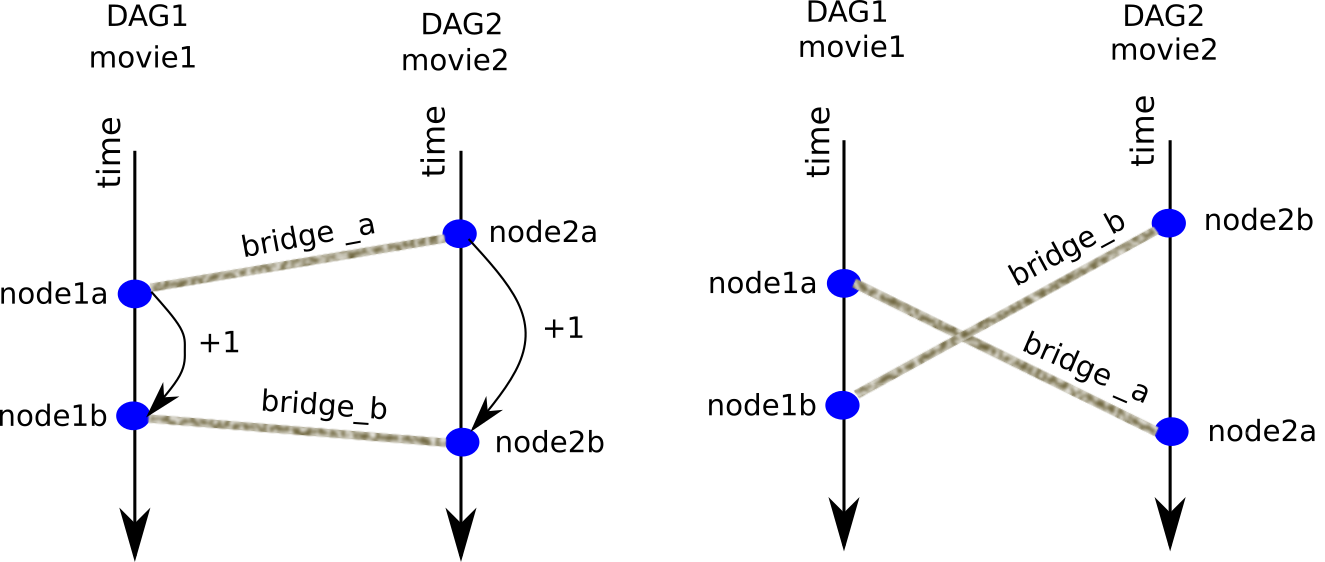
\includegraphics[width=5in]
{crossing-bridges.png}
\caption{Bridges span two DAGs (i.e., movies). We consider 2 possibilities:
bridges $a$ and $b$ cross,
or they don't. 
}
\label{fig-crossing-bridges}
\end{figure}

Next we consider every  pair $\{a,b\}$
of bridges. Suppose bridge  $a$ 
connects node $\tt node1a$ in movie 1
to node $\tt node2a$ in movie 2.
Likewise, suppose bridge $b$ connects
$\tt node1b$ in movie 1 to
node $\tt node2b$ in movie 2.
Let $\tt node1a.time$ be the time at which 
$\tt node1a$ occurs and define
$\tt node1b.time$,
$\tt node2a.time$, and
$\tt node2b.time$ similarly.
Assume that
$\tt
node1a.time< node1b.time$.
Then there are two possibilities
that we wish to consider. These 2 possibilities are illustrated in Fig.\ref{fig-crossing-bridges}.
Either the bridges don't cross 
(i.e. $a$ occurs before $b$ in both movies)
or they cross (i.e. $a$ occurs before $b$
in movie 1 but after in movie 2).
Let $N_{rep}$ be the {\bf number
of repetitions of an arrow}.
If bridges $a$ and $b$ cross,
we do nothing. If they don't cross,
we do the following for both DAG1 and DAG2.
If an arrow between the earlier and latter of the two nodes doesn't already
exist, we add it with $N_{rep}=1$.
If such an arrow already exists,
we increase its $N_{rep}$ by one.

That's basically the whole algorithm.
At the end of it, we will have
generated DAG1 for movie 1 and DAG2 for movie 2.

When drawing one of those DAGs,
one specifies a number {\tt reps\_threshold}$=N_{reps}^*$.
Only the arrows with $N_{reps}> N^*_{reps}$
are drawn.
The number $N_{reps}$ for each arrow is drawn
in the middle of the arrow.




\begin{figure}[h!]
\centering
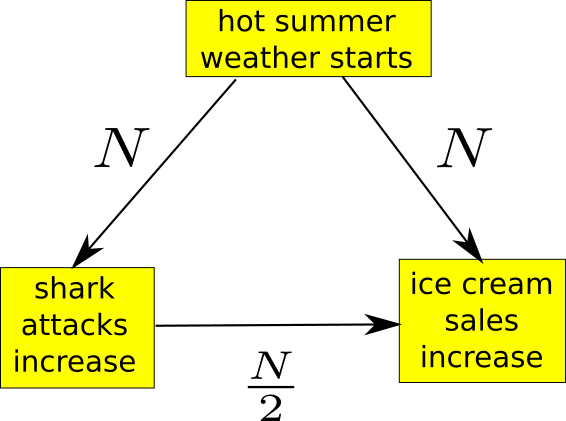
\includegraphics[width=2in]
{shark-attacks.png}
\caption{
DAG that expresses the fact that both
shark attacks and ice
cream sales increase during the summer,
because both are caused by hot summer weather.
}
\label{fig-shark-attacks}
\end{figure}

Here is a simple argument for
why this algorithm should work.
Consider Fig.\ref{fig-shark-attacks}.
The figure depicts a DAG that
expresses the fact that both
shark attacks and ice
cream sales increase during the summer,
because both are caused by hot summer weather.
Let 

$H$ = hot summer weather starts,

$Sh$ = shark attacks increase, 

$IC$ = ice cream sales increase.

If we compare this DAG to $N$
other DAGs that contain these 3 nodes,
then, since it is always true
that summer precedes shark
attack increases and ice cream sales increases, the two arrows 
emanating
from the $H$ node 
will have $N_{reps} =N$.
On the other hand, we expect that half of the time, the $Sh$ node will occur before
the $IC$ node,
and half of the time it will happen after.
Hence, $N_{reps}=\frac{N}{2}$ for the
arrow $Sh\rarrow IC$.

Let $\tt reps\_threshold$ $=N_{reps}^*$. Select $N_{reps}^*$ such that
$\frac{N}{2}< N_{reps}^* < N$. If when we draw this DAG, 
we only draw arrows with $N_{reps}> N_{reps}^*$, 
then only the two causal arrows will be visible. The difference  between
 $N_{reps}$ for the causal and non-causal
 arrows (call it the {\bf repetition gap})
  will grow 
   as $\frac{N}{2}$.
   
   
 It's important to point out
 that I expect this algorithm
 to produce good DAGs only
 after a large number $N$ of DAGs (i.e.,
 movie scripts or short stories)
 are compared. That's because the repetition gap
 grows relatively slowly, just linearly in $N$. Since,
 due to lack of hardware resources,
 this paper
 only compares a minuscule $N=3$,
 one can't expect very dramatic causal
 revelations from this paper.

It's also important to point out
that every time a new movie script is added to
the list of the $N$ already
analyzed movie scripts,
that new movie script must be compared to the
preceding $N$ movie scripts.
If we imagine a robot watching a movie daily,
then his daily dream time, if used solely
for movie comparison, 
would grow linearly in time.
At some point, it would take more than a day
of dream time to
compare today's movie to all movies in its past.
To keep his dream time constant, at 8 hours a day,
the robot
would have to compare today's movie
to a fixed number, say the most recent 365 movies 
viewed previously.

This section has described how the original version 
of MM did DEFT. More recent versions
of MM do DEFT slightly differently. For each arrow, the new versions store two weights $n_{acc}$
and $n_{rej}$ instead of just one weight $N_{reps}$.
As we explain in Appendix \ref{app-2-weights}, this
2 weight per arrow DEFT is stricter and more 
specific.




 

\section{Software Description}

The full MM process applied to the 3 short stories,
is documented in the jupyter notebook

$$\tt jupyter\_notebooks/navigating\_short\_stories.ipynb$$

The full MM process applied to the 3 movie scripts,
is documented in the jupyter notebook

$$\tt jupyter\_notebooks/navigating\_m\_scripts.ipynb$$

For a detailed description, encompassing 
every method and variable used in the
MM software,
please consult the software's Python ``docstrings".
This section of the paper merely
presents a brief overview of what you
will find in those jupyter notebooks and docstrings.

The full process from raw data to DAG atlas
is broken down in MM to
performing the following steps. 
Most of my time programming
was spent on the scripts that do
pre-processing of the data (
i.e., steps 2, 3 and 4 below).
Pre-processing data is hard!,
and not doing it is fatal
to this algorithm. When 
evaluating the similarity between
two ssents,
even small misspellings can 
change that value substantially.
 

\begin{enumerate}
\item Data scraping using methods in $\tt downloading\_imsdb.py$.

This python script was only used for the movie
scripts, not for the short stories. It 
scrapes all the movie scripts from the IMSDb
website using the Python package Beautiful Soup.

\item Cleaning using methods in $\tt cleaning.py$

Here I remove contractions like ``didn't",
and replace exclusively unicode symbols 
by their closest ANSII analogues (e.g.,
curly quotes are replaced by straight quotes).

Here I also use the software SpaCy\footnote{In the Python
world, there are 2 general, dominant
NLP libraries, SpaCy and NLTK (Natural Language Tool Kit). MM uses both. There is much overlap
between the 2. In case of overlap, I tried to use the one that was fastest.} to break up the movie script into 
separate sentences, and return a file with only
one sentence per line.

For the case of movie scripts (but not for short 
stories), I also try to distinguish between 
dialog lines and narration lines.
In many but not all movie scripts, the dialog lines are indented with 
respect to the narration lines.
In the case of Pixar/Disney, they don't indent dialog. In cases where the movie script indents,
the MM software gives the option of throwing away all the dialog lines and keeping only the narration
ones.



\item Spell-checking using methods in $\tt spell\_checking.py$

I discovered, to my chagrin, that spell-checking
without any input from a human user,
is very error prone, unless one takes context into consideration. LLMs can do contextual spell-checking, but this project did not use LLMs,
since I don't have access to them.
Instead of a contextual spell-checker,
I used the non-contextual
spell-checker $\tt pyspellchecker$
that tries to replace infrequent words by
more frequent ones (a very risky
and error prone approach). To 
diminish the risk, I
 constrained it in various ways so
that it only makes very conservative corrections.

\item Simplifying using methods in $\tt simplifying.py$

At this point, the file
has only one
full sentence per line.
Here, I  use Openie6 to
break each full sentence into ssents.\footnote{Alternatively,
one can use my software SentenceAx.
SentenceAx is a full rewrite of Openie6. 
Openie6 and SentenceAx are both available at GitHub.
}
Each line with a full sentence is replaced by
all of ssents derived from the full sentence.  The
ssents are separated by 
a separator-token ({\tt ZTZ\_SEPARATOR}).


Each ssent becomes a node of the DAG.

If  a ssent (i.e., node) appears at the
row $t$ of the file (counting starting with 0), then 
we say that node occurs at time $t$. If a ssent appears after zero separator-tokens, we say $x=0$ for it.
If it appears after one separator-token, we say $x=1$ for it, and so forth. Hence each node (i.e., ssent)
can be labeled by its $(t,x)$ coordinates.


\item Creating DAG atlas using methods in
$\tt DagAtlas.py$

Everything up to this point has just been
pre-processing of the data. 
Here, I finally implement the algorithm described
in Section \ref{sec-algo-overview}.
The bottleneck and rate-determining-step for
the full MM process is
calculating the similarity between 2 nodes.
If DAG1 for movie script (or short story) 1 has $k_1$ 
nodes, and DAG2 has $k_2$ nodes,
then $k_1 k_2$ similarity calculations have to be made.
For the short stories I considered, $k_1k_2$
is typically on the order of $0.1M$.
For the movies, it is typically $1.5M$.

For the similarity measure between nodes (i.e., ssents), I tried 
many methods. I
ended up using sBERT. 

\item Visualizing DAGs using methods in $\tt Dag.py$.

This step is easy. I use $\tt graphviz$ to 
accomplish it.

\end{enumerate}

\section{Possible Improvements
of the MM algorithm
using LLMs}

MM uses 
LLMs twice: first, 
it uses Openie6
to do sentence spitting,
and second, it uses 
sBERT to calculate sentence
similarities.
Openie6 and sBERT are both
fine tunings of BERT.
BERT is the encoder 
part of the Vanilla Transformer
Network
first proposed in 2017.\footnote{For more information about Transformer Networks,
see my book Bayesuvius (Ref.\cite{bayesuvius}) which
has a long chapter dedicated
to them.}


MM does not, however, use 
a promptable LLM such as
ChatGPT. But it could use one.
A promptable
LLM could perform
the 3 data pre-processing steps
(2-cleaning, 3-spell-checking and 4-simplifying) in lieu of 
Openie6. It could also calculate sentence similarities in lieu of sBERT.


To demonstrate that 
promptable LLMs can 
perform these task superbly, I
did the following test. I gave ChatGPT the
beginning narrative paragraph of the movie 
WALL-E, and I asked her to summarize the
paragraph as a list of simple declarative sentences.
Here is the result:
\\
\hrule
\noindent {\bf PROMPT:} 

Consider the following quote:
\begin{quote}
``A range of mountains takes form in the haze.
Moving closer.
The mountains are piles of TRASH.
The entire surface is nothing but waste.

``..We're gonna find adventure in the evening air...''

A silhouetted city in the distance.
What looks like skyscrapers turns into trash.
Thousands of neatly stacked CUBES OF TRASH, stories high.
Rows and rows of stacked cubes, like city avenues.
They go on for miles."
\end{quote}

Give an enumerated list summarizing this quote.
Each list item must be a simple declarative sentence
consisting of a subject phrase and a verb phrase.
The list items must be in chronological order of occurrence
in the quote.
\\
\hrule
\noindent {\bf REPLY:}

\begin{enumerate}
\item A range of mountains appears in the haze.
\item The narrator moves closer.
\item The mountains are revealed to be piles of trash.
\item The entire surface is described as nothing but waste.
\item The narrator speaks of finding adventure in the evening air.
\item A silhouetted city appears in the distance.
\item The skyscrapers turn out to be made of trash.
\item Thousands of neatly stacked cubes of trash are seen, stories high.
\item Rows and rows of stacked cubes are seen, resembling city avenues.
\item The expanse of trash goes on for miles.
\end{enumerate}
\hrule
.\\
Each of these 10 sentences would make
a superb node in a causal DAG. With nodes defined
with such clarity, 
one could avoid much noise in the calculation of the similarity
of 2 nodes.


\section{Possible Improvements
of LLMs 
using the MM algorithm}
 
LLMs
are very good at what they do,
but ultimately, they are just curve fitters
that cannot perform the scientific method (SM)
and causal inference (CI)
in a deliberate way. At best, they can 
perform the SM in a trial an error way, as in 
Fig.\ref{fig-harris-e-mc2}.
This weakness of LLMs can be overcome
by adding to them
a DAG atlas and an explicit (not an implicit or emergent) CI engine.


\begin{figure}[h!]
\centering
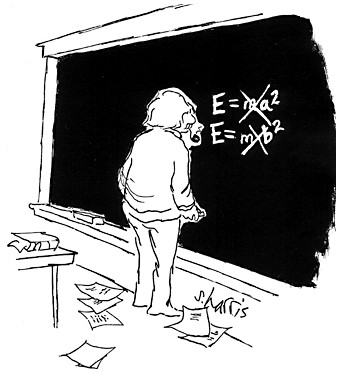
\includegraphics[width=3in]
{harris-e-mc2.jpg}
\caption{Cartoon 
by S.Harris
about $E=mc^2$.
}
\label{fig-harris-e-mc2}
\end{figure}

\appendix

\section{Appendix: Two weights per arrow instead of one}\label{app-2-weights}

In the original MM version, each arrow carries a single weight $N_{reps}$ initially set to 0. $N_{reps}=$ the number
of repetitions of that arrow. When we compare two bridges,
\begin{itemize}

\item If the bridges don't
cross, we increase by 1 the $N_{reps}$
 for the arrow between points $a$ and $b$ in
movie 1, and for the
corresponding arrow in movie 2.

\item
If the bridges cross, we do nothing. 
\end{itemize}
We then define a threshold value $N^*_{reps}$
for $N_{reps}$.
When drawing the DAG, we only
draw arrows with $N_{reps}>N^*_{reps}$.
Each arrow in the DAG looks like 

$$\xymatrix@C=5pc{A\ar[r]_5&B}$$
when $N_{reps} =5$


In the new version of MM, 
each arrow carries a pair of weights $(n_{acc}, n_{rej})$ initially set to $(0,0)$.
$n_{acc}=$ the number of acceptances.
$n_{rej}=$ the number of rejections. 

\begin{itemize}
\item If the bridges don't
cross, we accept. We increase $n_{acc}$ by 1, for the arrow between bridges $a$ and $b$ in movie 1,
and for the corresponding arrow in movie 2. 
\item
If the bridges cross, we reject. We increase $n_{rej}$ by 1, for the arrow between bridges $a$ and $b$ in movie 1,
and for the corresponding arrow in movie 2. 
\end{itemize}

We define the acceptance probability $p_{acc}$ 
for each arrow by

\beq
p_{acc} = \frac{n_{acc}}{n_{acc} + n_{rej}}
\eeq
We also define the total number $N$ of samples for each arrow by

\beq
N = n_{acc} + n_{rej}
\eeq
Then we  define a threshold value $p^*_{acc}$ 
for $p_{acc}$ and a threshold value $N^*$
for $N$. When drawing the DAG, we only draw arrows with $p_{acc}>p^*_{acc}$
and $N> N^*$. Each arrow in the DAG looks like 

$$\xymatrix@C=5pc{A\ar[r]_{0.93 (5)}&B}$$
when $p_{acc} =0.93$ and $N= 5$.

\begin{figure}[h!]
\centering
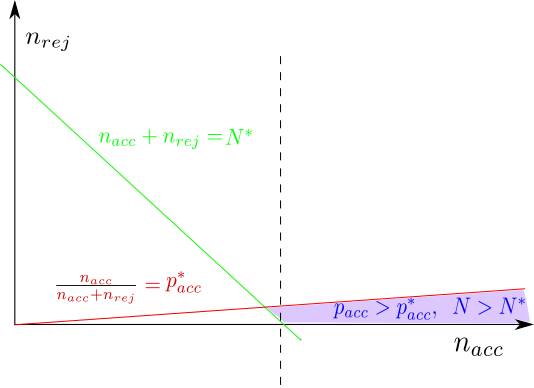
\includegraphics[width=4in]
{nacc-nrej-plane.png}
\caption{
$(n_{acc}, n_{rej})$ plane. The purple region satisfies the 
2 constraints $p_{acc} > p_{acc}^*$ and $N> N^*$.}
\label{fig-nacc-nrej-plane}
\end{figure}


Fig.\ref{fig-nacc-nrej-plane}
shows a picture of the $(n_{acc}, n_{rej})$
plane. We assume that $p_{acc}^*$ is fairly
close to 1 so the
line $\frac{n_{acc}}{n_{acc}+ n_{rej}} = p^*_{acc}$
is close to being horizontal.
The purple region satisfies the 
2 constraints $p_{acc} > p_{acc}^*$ and $N> N^*$.

The two weights per arrow (2W/A) method
gives bnets with fewer  but more trustworthy
arrows, than the one weight per arrow (1W/A) method. 
This can be easily seen from Fig.\ref{fig-nacc-nrej-plane}.
The $N_{reps}$ in the 1W/A method corresponds to
the $n_{acc}$ in the 2W/A method.
Thus, the threshold $N^*_{reps}$ for $N_{reps}$
becomes a threshold $n^*_{acc}$ for $n_{acc}$.
The set of points satisfying $n_{acc} > n^*_{acc} $
equals a half plane $H$ in $(n_{acc}, n_{rej})$ space. For instance, if $n_{acc}^*$
is the value of $n_{acc}$
for the dashed line 
in Fig.\ref{fig-nacc-nrej-plane},
then $H$ equals the half plane of all points to the right of that
dashed line.
Clearly, $H$
contains many more 
points than the purple region
in Fig.\ref{fig-nacc-nrej-plane}.

Hence, one is justified in saying that the 2W/A method
is stricter and more specific (i.e., more restrictive) than the
1W/A method. It is also
less lossy. When the 1W/A method does nothing 
for crossing bridges, it is
throwing away some information
that the 2W/A method keeps. This extra information
is used to filter out less trustworthy points with
high $n_{rej}$ counts (high compared to $n_{acc}$)







\bibliographystyle{plain}
\bibliography{references}
\end{document}
